\documentclass[a4paper]{article}

\usepackage[utf8x]{inputenc}    
\usepackage[T1]{fontenc}
\usepackage[spanish]{babel}
\usepackage{multicol}

\usepackage{wrapfig}
\usepackage{graphicx}

\usepackage{bm}
\usepackage{amsxtra} 
\usepackage{amssymb}% to get the \mathbb alphabet
\usepackage{amsmath}

\usepackage[box,completemulti,separateanswersheet]{automultiplechoice}    
\def\AMCformQuestion#1{\vspace{\AMCformVSpace}\par {\sc Pregunta #1:} }    
\def\AMCbeginQuestion#1#2{\par\noindent{\bf Pregunta #1}#2\hspace*{1em}}
\def\AMCcleardoublepage{\ifodd\thepage\clearpage\mbox{}\fi\clearpage}

\begin{document}

\AMCrandomseed{1237893}

%%%%%%%%%%%%%%%%%%%%%%%%%%%%%%%%%%%%%%%%%%%%%%%%%%%%%%%%%%%%%%%%%%%%%%%%%%%%%
\element{test1}{
\begin{question}{p1}
El caudal que se filtra, en régimen estacionario, a la salida del túnel vale aproximadamente:
\begin{multicols}{2}
\begin{choices}
	\correctchoice{$33.7$ l/s}
	\wrongchoice{$4.21$ l/s}
	\wrongchoice{$156.1$ l/s}
	\wrongchoice{$21.01$ l/s}
\end{choices}
\end{multicols}
\end{question}
}
%%%%%%%%%%%%%%%%%%%%%%%%%%%%%%%%%%%%%%%%%%%%%%%%%%%%%%%%%%%%%%%%%%%%%%%%%%%%%
\element{test1}{
\begin{question}{p2}
El valor mínimo de la altura piezométrica se alcanza en:
\begin{multicols}{2}
\begin{choices}
	\correctchoice{La salida del túnel}
	\wrongchoice{Un punto de contacto del dique con el suelo 2}
	\wrongchoice{La zona de contacto del agua con el medio 1}
	\wrongchoice{La zona de contacto del agua con el suelo 2}
\end{choices}
\end{multicols}
\end{question}
}
%%%%%%%%%%%%%%%%%%%%%%%%%%%%%%%%%%%%%%%%%%%%%%%%%%%%%%%%%%%%%%%%%%%%%%%%%%%%%
\element{test1}{
\begin{question}{p3}
El valor máximo de la altura piezométrica se alcanza en:
\begin{multicols}{2}
\begin{choices}
	\correctchoice{La zona del suelo 1 situada entre la pantalla izquierda y el dique, en contacto con el agua}
	\wrongchoice{La zona del suelo 2 situada entre el dique y la pantalla derecha, en contacto con el agua}
	\wrongchoice{La parte superior de la salida del túnel}
	\wrongchoice{La parte inferior de la salida del túnel}
\end{choices}
\end{multicols}
\end{question}
}
%%%%%%%%%%%%%%%%%%%%%%%%%%%%%%%%%%%%%%%%%%%%%%%%%%%%%%%%%%%%%%%%%%%%%%%%%%%%%
\element{test1}{
\begin{question}{p4}
Los valores de la velocidad vertical están comprendidos aproximadamente entre:
\begin{multicols}{2}
\begin{choices}
	\correctchoice{$-65$ y $5$ mm/s}
	\wrongchoice{$0$ y $3.5$ mm/s}
	\wrongchoice{$-100$ y $0$ mm/s}
	\wrongchoice{$-25$ y $25$ mm/s}
\end{choices}
\end{multicols}
\end{question}
}
%%%%%%%%%%%%%%%%%%%%%%%%%%%%%%%%%%%%%%%%%%%%%%%%%%%%%%%%%%%%%%%%%%%%%%%%%%%%%
\element{test1}{
\begin{question}{p5}
Los valores de la velocidad horizontal están comprendidos aproximadamente entre:
\begin{multicols}{2}
\begin{choices}
	\correctchoice{$-25$ y $50$ mm/s}
	\wrongchoice{$-10$ y $100$ mm/s}
	\wrongchoice{$0$ y $50$ mm/s}
	\wrongchoice{$-50$ y $0$ mm/s}
\end{choices}
\end{multicols}
\end{question}
}
%%%%%%%%%%%%%%%%%%%%%%%%%%%%%%%%%%%%%%%%%%%%%%%%%%%%%%%%%%%%%%%%%%%%%%%%%%%%%
\element{test1}{
\begin{question}{p6}
El valor de $h$ en el punto A vale:
\begin{multicols}{2}
\begin{choices}
	\correctchoice{$7.3$ m}
	\wrongchoice{$1.2$ m}
	\wrongchoice{$2.9$ m}
	\wrongchoice{$5.1$ m}
\end{choices}
\end{multicols}
\end{question}
}
%%%%%%%%%%%%%%%%%%%%%%%%%%%%%%%%%%%%%%%%%%%%%%%%%%%%%%%%%%%%%%%%%%%%%%%%%%%%%
\element{test1}{
\begin{question}{p7}
El valor de la presión de poro, $p_w$, en el punto B, vale:
\begin{multicols}{2}
\begin{choices}
	\correctchoice{$47.6$ KPa}
	\wrongchoice{$7.1$ KPa}
	\wrongchoice{$121.6$ KPa}
	\wrongchoice{$0.50$ KPa}
\end{choices}
\end{multicols}
\end{question}
}
%%%%%%%%%%%%%%%%%%%%%%%%%%%%%%%%%%%%%%%%%%%%%%%%%%%%%%%%%%%%%%%%%%%%%%%%%%%%%
\element{test1}{
\begin{question}{p8}
El valor de la velocidad de flujo horizontal en el nodo superior de la salida del túnel vale:
\begin{multicols}{2}
\begin{choices}
	\correctchoice{$47.8$ mm/s}
	\wrongchoice{$-1.26$ mm/s}
	\wrongchoice{$7.45$ mm/s}
	\wrongchoice{$-45.5$ mm/s}
\end{choices}
\end{multicols}
\end{question}
}

%%%%%%%%%%%%%%%%%%%%%%%%%%%%%%%%%%%%%%%%%%%%%%%%%%%%%%%%%%%%%%%%%%%%%%%%%%%%%
\element{test1_b}{
\begin{question}{p8-b}
El valor de la fuerza de subpresión en el dique vale:
\begin{multicols}{2}
\begin{choices}
	\correctchoice{$48.7$ kN}
	\wrongchoice{$5.71$ kN}
	\wrongchoice{$138.2$ kN}
	\wrongchoice{$117.3$ kN}
\end{choices}
\end{multicols}
\end{question}
}
%%%%%%%%%%%%%%%%%%%%%%%%%%%%%%%%%%%%%%%%%%%%%%%%%%%%%%%%%%%%%%%%%%%%%%%%%%%%%
\element{test1}{
	\begin{question}{p9}
		En un problema de conducción de calor, la condición natural de contorno:
		$$\bm{q} \cdot \bm{n} = \overline{q}, \textrm{ en } \partial_t \Omega$$
		se interpreta como:
		\begin{multicols}{2}
			\begin{choices}
				\correctchoice{El valor impuesto, de tipo escalar, que corresponde al
					flujo de calor en dirección normal al contorno $\partial_t \Omega$}
				\wrongchoice{El valor impuesto, de tipo vectorial, que corresponde al
					flujo de calor en el contorno $\partial_t \Omega$}
				\wrongchoice{El valor impuesto, de tipo escalar, que corresponde al
					gradiente de la temperatura en dirección normal al contorno $\partial_t \Omega$}
				\wrongchoice{El valor impuesto, de tipo vectorial, que corresponde al
					gradiente de la temperatura en el contorno $\partial_t \Omega$}
			\end{choices}
		\end{multicols}
	\end{question}
}
%%%%%%%%%%%%%%%%%%%%%%%%%%%%%%%%%%%%%%%%%%%%%%%%%%%%%%%%%%%%%%%%%%%%%%%%%%%%%
\element{test1}{
	\begin{question}{p10}
		El concepto de compatibilidad, en el ámbito del método de los elementos finitos,
		establece:
		\begin{multicols}{2}
			\begin{choices}
				\correctchoice{Un requisito de continuidad de las funciones de forma,
					entre elementos adyacentes}
				\wrongchoice{Un requisito de continuidad de las funciones de forma,
					en el interior de los elementos}
				\wrongchoice{Que cuando el tamaño de los elementos tiende a $0$,
					la solución aproximada prácticamente coincide con la solución exacta del
					problema de contorno}
				\wrongchoice{Que el valor de la suma de las funciones de forma de un
					elemento es igual a $1$}
			\end{choices}
		\end{multicols}
	\end{question}
}

%%%%%%%%%%%%%%%%%%%%%%%%%%%%%%%%%%%%%%%%%%%%%

\scoringDefaultS{b=1,m=-1/(N-1)}

\onecopy{1}{    

%%% beginning of the test sheet header:    

\noindent{\large\bf Método de los Elementos Finitos  \hfill MUECYM \hfill TEST \# 2}
\begin{center}
%\vspace*{.1cm}
%Se atribuirá puntuación negativa a las respuestas incorrectas.\\
\vspace*{.1cm}
25 nov 2024. \hspace{7cm} Tiempo: 60 minutos.\\


\end{center}

\vspace{1ex}

La figura muestra la sección transversal de un río canalizado (de 1 m de espesor), limitado por dos pantallas impermeables. En el interior, se encuentra un dique impermeable cimentado sobre el suelo. La geometría del río, dique, pantallas y distribución de las diferentes permeabilidades de los suelos se muestra en la figura a continuación.\\

En la zona derecha inferior se ha dejado abierto un espacio, de 1 m de altura, sometido a la presión atmosférica.\\

El suelo 1 tiene un coeficiente de permeabilidad $k_1 = 10^{-3}$ m/s. El suelo 2 tiene un coeficiente de permeabilidad $k_2 = 3 \cdot 10^{-3}$ m/s y el suelo 3 $k_2 = 2 \cdot 10^{-2}$ m/s.\\

Para analizar las filtraciones que se producen se realizará un modelo plano de elementos finitos que represente dicha sección transversal. La discretización a efectuar corresponde a elementos rectangulares lineales de cuatro nodos (DC2D4) de lado apróximado 0,30 m. Considerar la opción de forma de elemento \emph{Quad Dominated}, y con técnica tipo \emph{Free}.\\

\textbf{NOTA: Para homogeneizar los valores de la altura piezométrica se tomará como altura geométrica z = 0 la de los puntos del terreno impermeable}\\

\begin{center}
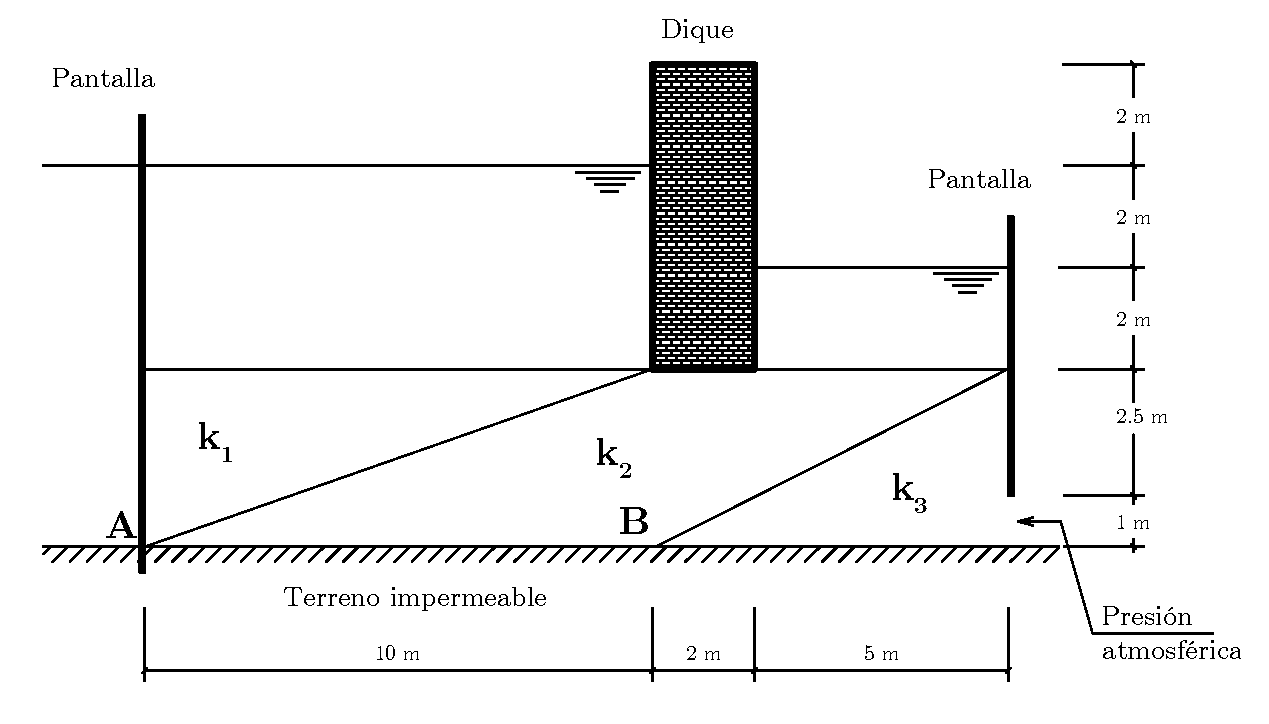
\includegraphics[width=0.90\textwidth]{ejerc2}
\end{center}

\hrulefill
\vspace{4mm}

%%% end of the header

\shufflegroup{test1}
\insertgroup{test1}

%\AMCcleardoublepage    
\clearpage

\AMCformBegin    

%%% beginning of the answer sheet header

\noindent\AMCcode{nummat}{2}\hspace*{\fill}
\begin{minipage}{.7\linewidth}
$\longleftarrow{}$ Escriba su número de matrícula marcando los dígitos
en los recuadros (con ceros a la izquierda si el número es de menos de dos dígitos) y el nombre y apellidos debajo.

\vspace{3ex}

\namefield{\fbox{
   \begin{minipage}{.9\linewidth}
     Apellidos, Nombre:

     \vspace*{.5cm}\dotfill
     \vspace*{1mm}
   \end{minipage}
 }}
\end{minipage}

\begin{center}
 \bf\em Debe dar las respuestas exclusivamente en esta hoja (las respuestas en las demás hojas no serán tenidas en cuenta).
\end{center}

%%% end of the answer sheet header


\AMCform    

%\AMCcleardoublepage    

}  

\end{document}
